%% -*- coding:utf-8 -*-
\begin{figure}
\centering

\ifpdf
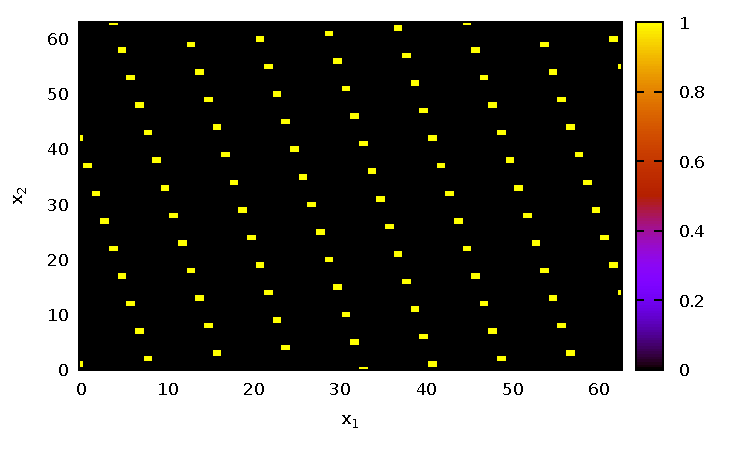
\includegraphics[angle=0]
{./part4/quantcomp/picellipticdiscretlog1.pdf}
\else
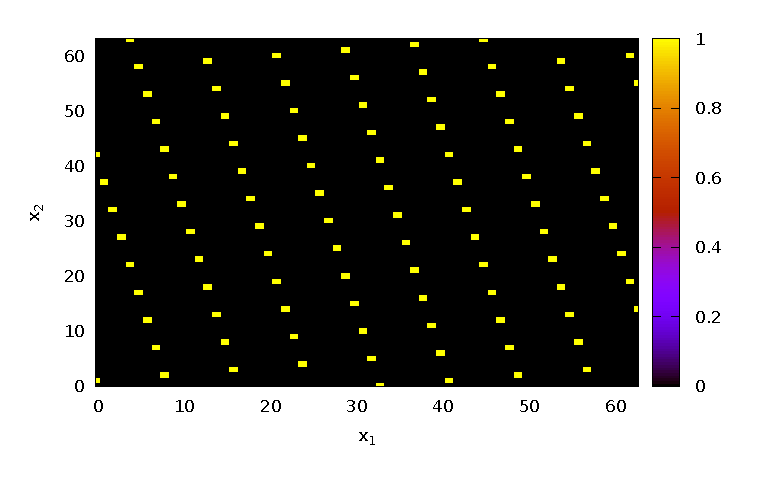
\includegraphics[angle=0]
{./part4/quantcomp/picellipticdiscretlog1.eps}
\fi

%\input ./part4/quantcomp/picdiscretlog2.tex

%% *Elliptic> c = Curve (-7) 10 97
%% *Elliptic> g = Point 96 93 c
%% *Elliptic> aa = Point 37 35 c
%% *Elliptic> filter (\(x1,x2) -> (1 .*. aa) .+. (2 .*. g) == g) [(x1,x2) | x1 <- [0..20], x2 <- [0..10]]
%% []
%% *Elliptic> filter (\(x1,x2) -> (x1 .*. aa) .+. (x2 .*. g) == g) [(x1,x2) | x1 <- [0..20], x2 <- [0..10]]
%% [(0,1),(7,7),(8,2),(15,8),(16,3)]


\caption{График функции 
$f'(x_1, x_2)$ при $x_0 = 1$. Т.о. изображены точки $x_1, x_2$
  соответствующие соотношению $x_1 A + x_2 g = g$: 
  $x_1 (37, 35) + x_2 (96,93) = (96,93)$, например
  $7 (37, 35) + 7 (96,93) = (96,93)$ или $8 (37, 35) + 2 (96,93) = (96,93)$} 
\label{fig:part4:quantcomp:dle1}
\end{figure}
